\subsection{Kill-First-AI}
We thought of various ways to implement AI agents for the game. Our final AI implementation is based on the decision tree model. The logic behind the implementation is illustrated in Figure \ref{fig:tree1}.

\begin{figure}
\centering
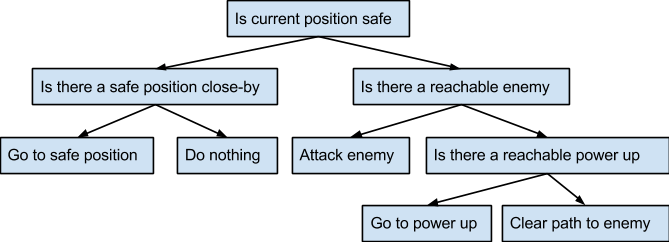
\includegraphics[width=10cm]{resources/tree1}
\caption{Decision Tree}
\label{fig:tree1}
\end{figure}

As you can see the logic behind the AI agents is relatively simple, in a step by step breakdown of the figure above we see the states of the agent being divided into two different categories. One is the case in which the current position of the agent is safe and the agent has time to plot it’s  next move and the other is when the agents position is threatened by a bomb. This is the major concern of the agent when checking for the next move. 
In case the current position is threatened by a close-by bomb or the player is located on a bomb (in our implementation of the game this can only occur after it itself has placed it), the player looks for a way to avoid the threat by moving away from the bomb. If looking for a safe position returns no viable results then there is nothing to do and the player loses. If not the player will follow the path returned to him by the ‘findClosestSafeSpot()’ method.
On the other subtree we see the tactics the bot will make use of in order to achieve his goal in defeating his opponents. The ‘isEnemyReachable()’ function will return whether if the closest opponent to the player is within reach, meaning if there is no obstacle in the path returned using the A* algorithm. If there is at least one obstacle in that path then the bot assumes that there is still time to pick up power-ups instead and focuses on that. Furthermore the instant the enemy becomes reachable, the bot’s top priority becomes attacking the opponent instead.


\subsubsection{Attacking Tactics}
Attacking the enemy can be achieved in various ways. Initially our tactic was the following: if the player has an opponent within 3 blocks away from him then he would place a bomb in order to attack him. Later on during the evaluation process we thought that we could introduce the concept of the bot already knowing the firepower it has in it’s disposal. That is how we came up with the final simple approach which was the following: if the bot has a player within reach (with respect to the bot’s firepower) then it will place a bomb to attack them.

Moving and Path Finding Tactics
Pulling up the Map class had a lot of positive impact in making the moving of the players easier. This enabled us to make use of all the functions necessary to implement path finding algorithms. The path finding algorithm we made use of was the A* algorithm. At this point we had to determine the costs of moving through the various types of blocks in the map. We have three types of map cells in the map those are the following :
\begin{itemize}
\item Empty spaces
\item Obstacles
\item Walls
\end{itemize}

Obviously the empty spaces and walls have trivial scores of 1 and undefined (infinity) respectively. However, the one that took some effort in order to figure out, was the obstacle cost.
Initially the players will have obstacles between them and still would require to calculate the distances between them. The final cost we assigned to the ‘obstacle’ class of map cell finally was 4. We observed some weird behaviours when this score was 3. That is the bots would end up trapped by their bombs after placing them. We assumed that the difference between 3 and 4 is that when the cost is fixed to 4 the bot prefer moving around an obstacle more to blasting through it. That is the reason why it will never try to reach a safe position after placing a bomb by blasting it’s way through another obstacle.

\subsection{Upgrade-First-AI}
\todo{Explain this AI here}
